\documentclass{article}

\usepackage{/home/paul/Workspace/build/macros}


\title{Annale 2024: corrigé}
\date{}
\author{Paul Catala}


\begin{document}
\maketitle

\section{Optimisation numérique}

\subsection{Questions de cours}

\begin{enumerate}
	\item 
	\begin{enumerate}
		\item Les variables du problème sont $x_1$ et $x_2$
		\item La fonction objectif du problème est $f(x_1,x_2) = (x_1-3)^2 + (x_2+2)^2$
		\item Le problème a deux contraintes: une contrainte d'égalité $3x_2^2-x_1=0$, et une contrainte d'inégalité $x_1+x_2 \leq 2$
		\item La contrainte d'égalité peut se reformuler $x_1 = 3x_2^2$, et donne l'expression de $x_1$ en fonction de $x_2$. On peut donc reformuler le problème en fonction de $x_2$ uniquement. En réinjectant dans le problème ($\Pp$), on obtient le nouveau critère
		\eq{\begin{aligned}
			g(x_2) = (3x_2^2 - 3)^2 + (x_2+2)^2 &= 9x_2^4 - 18x_2^2 + 9 + x_2^2 + 2x_2 + 2\\
			&= 9x_2^4  - 17x_2^2 + 2x_2 + 11
			\end{aligned}
		}
		et la nouvelle contrainte
		\eq{
			3x_2^2+x_2 \leq 2
		}
		Le problème est donc équivalent au nouveau problème
		\eq{\tag{$\Pp'$}
			\min_{x}  9x^4  - 17x^2 + 2x + 11 \quad\text{tel que}\quad x(3x+1) \leq 2
		}
	\end{enumerate}
	
	\item \begin{enumerate}
		\item Les variables sont $x_1,x_2$, la fonction objectif est $f(x_1,x_2) = 100(x_2-x_1^2)+(1-x_1)^2$, et il n'y a pas de contraintes.
		\item Soit $\mathbf{x}^* \eqdef (x_1^*,x_2^*) \in \RR^2$. Une condition nécessaire pour que $\mathbf{x}^*$ soit un minimiseur local est que le gradient de $f$ en $\mathbf{x}^*$ soit nul (si $f$ est de plus convexe, alors $\mathbf{x}^*$ est en fait un minuimiseur global).
		
		\item Calculons le gradient de $f$. On a
		\eq{
		f(x_1,x_2) = 100x_2^2 - 200x_1^2x_2 + 100x_1^4 + x_1^2 - 2x_1 + 1,
		}
		donc 
		\eq{
			\nabla f(x_1,x_2) = \begin{bmatrix} \partial_1 f (x_1,x_2) \\ \partial_2 f(x_1,x_2) \end{bmatrix} = \begin{bmatrix}-400x_1x_2 + 400x_1^3 + 2x_1 - 2 \\ 200x_2 - 400x_1^2 \end{bmatrix}.
		}
		En particulier,
		\eq{
			\nabla f(0,0) = \begin{bmatrix} -2 \\ 0\end{bmatrix}\neq \begin{bmatrix} 0 \\ 0 \end{bmatrix}
		}
		donc $[0,0]^\top$ n'est pas un minimiseur local du problème.
	\end{enumerate}
	
	\item \begin{enumerate}
		\item Une fonction $f$ est convexe si et seulement si
		\eq{
			\forall x,y, \quad \forall t\in[0,1],\quad f(tx+(1-t)y) \leq tf(x) + (1-t)f(y).
		}
		Autrement dit, toute corde prise entre deux points du graphe de $f$ est au-dessus du graphe de $f$.
		
		\item La fonction $(a)$ est convexe, mais pas strictement convexe: entre $-1$ et $1$, toute corde est confondu avec le graphe de la fonction (il y a égalité dans la définition précédente).
		
		La fonctioon $(b)$ est (strictement) convexe.
		
		La fonction $(c)$ n'est pas convexe.
		
		La fonction $(d)$ est (strictement) convexe.
		
		\item La convexité est une propriété intéressante en optimisation, car pour une fonction convexe, tout minimiseur local est en fait un minimiseur global (autrement dit, il n'y a que des minima globaux). On a donc de meilleures garanties de trouver le minimum global dans ce cas.
	\end{enumerate}
\end{enumerate}


\subsection{Moindres carrés linéaires}

\begin{enumerate}
	\item Le système (1) peut s'écrire sous forme matricielle comme
	\eq{
		\mathbf{y} = \mathbf{A}\mathbf{x} + \mathbf{b}
	}
	où
	\eq{
		\mathbf{y} = \begin{bmatrix}y_1\\y_2\\y_3\end{bmatrix}, \quad \mathbf{A} = \begin{bmatrix} 2 & 3 \\ 0 & 3 \\ 1 & 0\end{bmatrix}, \quad \mathbf{x} = \begin{bmatrix} x_1\\ x_2\\ x_3\end{bmatrix}, \quad \mathbf{b} = \begin{bmatrix} b_1 \\b_2 \\b_3 \end{bmatrix}.
	}
	
	$\mathbf{y}$ est le vecteur d'observations, $\xx$ est le vecteur d'inconnues, et $\mathbf{A}$ est la matrice de design.
	
	\item Puisque $\mathbf{y} = \mathbf{A}\mathbf{x}+\mathbf{b}$, on a donc $\norm{\mathbf{b}}_2 = \norm{\mathbf{A}\mathbf{x} - \mathbf{y}}_2$. Le problème d'optimisation que l'on cherche à résoudre est donc
	\eq{
		\min_{\mathbf{x}\in\RR^3} \norm{\mathbf{A}\mathbf{x}-\mathbf{y}}_2.
	}
	En pratique on minimise plutôt la normé euclidienne au carré (ce qui est équivalent)
	\eq{
		\min_{\mathbf{x}\in\RR^3} \frac{1}{2}\norm{\mathbf{A}\mathbf{x}-\mathbf{y}}_2^2.
	}
	Ce problème s'appelle les moindres carrés linéaires.
	
	\item On a 
	\eq{\begin{aligned}
		\frac{1}{2}\norm{\mathbf{A}\mathbf{x} - \mathbf{y}}_2^2 
			= \frac{1}{2}(\mathbf{A}\mathbf{x}-\mathbf{y})^\top(\mathbf{A}\mathbf{x}-\mathbf{y})
			&= \frac{1}{2}\mathbf{x}^\top\mathbf{A}^\top \mathbf{A}\mathbf{x} - \mathbf{y}^\top \mathbf{A}\mathbf{x} + \frac{1}{2}\mathbf{y}^\top\mathbf{y}\\
			&= \frac{1}{2}\mathbf{x}^\top \mathbf{Q}\mathbf{x} + \mathbf{p}^\top \mathbf{x} + \mathbf{y}^\top\mathbf{y}
		\end{aligned}
	}
	où $\mathbf{Q} = \mathbf{A}^\top\mathbf{A}$ et $\mathbf{p} = -\mathbf{A}^\top \mathbf{y}$. En pratique le terme constant $\mathbf{y}^\top \mathbf{y}$ peut être ignoré lors de l'optimisation car il ne change pas le minimiseur. Le problème d'optimisation sous forme standard est donc
	\eq{
		\min_{\mathbf{x}\in\RR^3} \frac{1}{2}\mathbf{x}^\top \mathbf{Q}\mathbf{x} + \mathbf{p}^\top \mathbf{x}.
	}
	
	\item On appelle $f$ la fonction objectif. On a
	\eq{
		\nabla f(\mathbf{x}) = \mathbf{Q}\mathbf{x} + \mathbf{p}.
	}
	
	\item La fonction $f$ est quadratique, donc en particulier convexe, donc tout minimiseur local est global. Une condition nécessaire et donc ici suffisante d'optimalité est que le gradient soit nul. On en déduit que le minimiseur $\mathbf{x}^*$ doit ici satisfaire
	\eq{
		\mathbf{Q}\mathbf{x}^* = -\mathbf{p}.
	}
	Or
	\eq{
		\mathbf{Q} = \mathbf{A}^\top \mathbf{A} = \begin{bmatrix} 5 & 6 \\ 6 & 9 \end{bmatrix}
	}
	est inversible (le déterminant est non nul). On en déduit
	\eq{
		\mathbf{x}^* = -\mathbf{Q}^{-1}\mathbf{p},
	}
	soit
	\eq{
		\mathbf{x}^* = (\mathbf{A}^\top \mathbf{A})^{-1}\mathbf{A}^\top \mathbf{y} = \mathbf{A}^\dagger \mathbf{y}.
	}
	La matrice $\mathbf{A}^\dagger$ s'appelle la pseudo-inverse de $\mathbf{A}$.
\end{enumerate} 

\section{Classification}
\subsection{SVM à noyau}

\begin{enumerate}
	\item Le jeu de données est le suivant:
	\bigbreak
	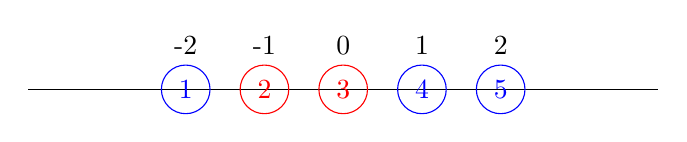
\begin{tikzpicture}
		\draw (-4,0) -- (4,0);
		
		\node[circle,blue,draw,label=-2] at (-2,0) {1};
		\node[circle,red,draw,label=-1] at (-1,0) {2};
		\node[circle,red,draw,label=0] at (0,0) {3};
		\node[circle,blue,draw,label=1] at (1,0) {4};
		\node[circle,blue,draw,label=2] at (2,0) {5};
	\end{tikzpicture}
	
	\item La séparabilité linéaire signifie ici que les deux classes sont de par et d'autre d'un point. Ce n'est pas le cas ici: les deux classes ne sont pas linéairement séparables.
	
	\item L'hyperplan suivant conduit à une erreur de classification, ce qui est bien le nombre minimal d'erreurs:
	\bigbreak
	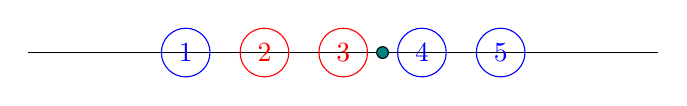
\begin{tikzpicture}
		\draw (-4,0) -- (4,0);
		
		\node[circle,blue,draw] at (-2,0) {1};
		\node[circle,red,draw] at (-1,0) {2};
		\node[circle,red,draw] at (0,0) {3};
		\node[circle,fill=teal,draw,inner sep=1.5pt] at (0.5,0) {};
		\node[circle,blue,draw] at (1,0) {4};
		\node[circle,blue,draw] at (2,0) {5};
	\end{tikzpicture}
	
	\item 
	\begin{enumerate}
		\item On a
		\eq{
			Z = \Phi(X) = \begin{bmatrix} X & X \odot X \end{bmatrix} = \begin{bmatrix} -2 & 4 \\ -1 & 1 \\ 0 & 0 \\ 1 & 1 \\ 2 & 4 \end{bmatrix}.
		}
		
		\item Graphiquement:
		\bigbreak
		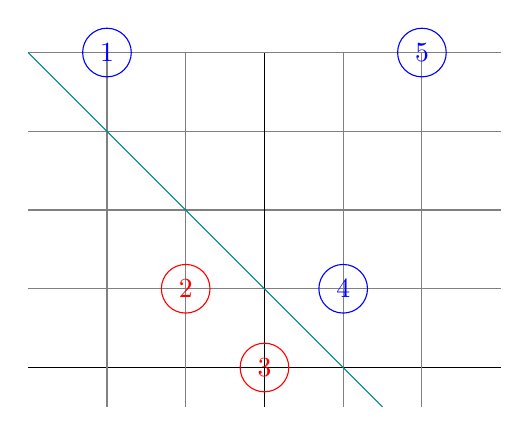
\begin{tikzpicture}
		\draw (-3,0) -- (3,0);
		
		\draw[gray] (-3,1) -- (3,1);
		\draw[gray] (-3,2) -- (3,2);
		\draw[gray] (-3,3) -- (3,3);
		\draw[gray] (-3,4) -- (3,4);
		
		\draw[gray] (-2,-0.5) -- (-2,4);
		\draw[gray] (-1,-0.5) -- (-1,4);
		\draw  (0,-0.5) -- (0,4);
		\draw[gray] (1,-0.5) -- (1,4);
		\draw[gray] (2,-0.5) -- (2,4);
		
		\draw[teal] (-3,4) -- (1.5,-0.5);
		
		\node[circle,blue,draw] at (-2,4) {1};
		\node[circle,red,draw] at (-1,1) {2};
		\node[circle,red,draw] at (0,0) {3};
		\node[circle,blue,draw] at (1,1) {4};
		\node[circle,blue,draw] at (2,4) {5};
	\end{tikzpicture}
	
	\item Les données sont bien linéairement séparables. Un hyperplan séparateur séparera les segments formées par les données $[x_1,x_4]$ et $[x_2,x_3]$. On vérifie graphiquement que ces segments sont parallèles, et que l'hyperplan séparateur à marge maximale est la droite parallèle à ces segments passant par le point de coordonnées (0,1). La marge est la distance entre les points $x_3$ et $x_4$, c'est-à-dire $\sqrt{2}$. 
	
	\item Il ya quatre vecteurs de support: $x_1$ et $x_4$ (pour la classe 1) et $x_2$ et $x_3$ (pour la classe -1). Ce sont toutes les données situées à la distance minimale de l'hyperplan.
	\bigbreak
	\begin{center}
		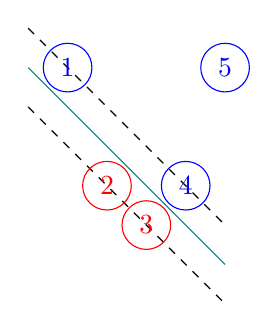
\begin{tikzpicture}
		\draw[teal] (-1.5,2) -- (1,-.5);
		
		\draw[dashed] (-1.5,1.5) -- (1,-1);
		\draw[dashed] (-1.5,2.5) -- (1,0);
		
		\node[circle,blue,draw] at (-1,2) {1};
		\node[circle,red,draw] at (-.5,0.5) {2};
		\node[circle,red,draw] at (0,0) {3};
		\node[circle,blue,draw] at (.5,0.5) {4};
		\node[circle,blue,draw] at (1,2) {5};
	\end{tikzpicture}
	\end{center}
	
	\item Si l'on retire la donnée $x_4$, qui est l'un des vecteurs de support, l'hyperplan séparateur change. Le nouvel hyperplan séparateur est parallèle à l'axe des abscisess et passe par (0,2.5), comme montré sur la figure ci-dessous. Les vecteurs $x_1$, $x_2$ et $x_3$ sont les nouveaux vecteurs de support. La nouvelle marge est $1.5$.
	
	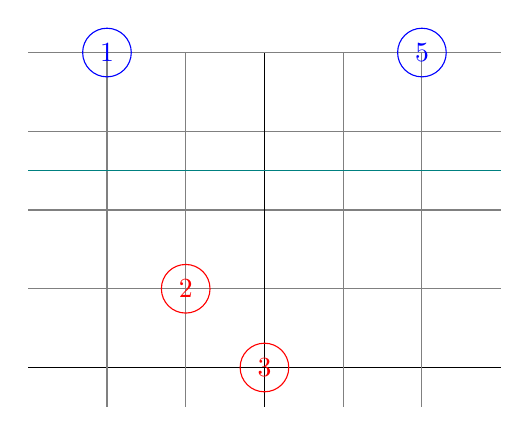
\begin{tikzpicture}
		\draw (-3,0) -- (3,0);
		
		\draw[gray] (-3,1) -- (3,1);
		\draw[gray] (-3,2) -- (3,2);
		\draw[gray] (-3,3) -- (3,3);
		\draw[gray] (-3,4) -- (3,4);
		
		\draw[gray] (-2,-0.5) -- (-2,4);
		\draw[gray] (-1,-0.5) -- (-1,4);
		\draw  (0,-0.5) -- (0,4);
		\draw[gray] (1,-0.5) -- (1,4);
		\draw[gray] (2,-0.5) -- (2,4);
		
		\draw[teal] (-3,2.5) -- (3,2.5);
		
		\node[circle,blue,draw] at (-2,4) {1};
		\node[circle,red,draw] at (-1,1) {2};
		\node[circle,red,draw] at (0,0) {3};
		\node[circle,blue,draw] at (2,4) {5};
	\end{tikzpicture}
	
	
	\end{enumerate}
	
	\end{enumerate}
	
	
	\section{Décompositions matricielles}
	
	\subsection{Valeurs propres et valeurs singulières}
	
	\begin{enumerate}
		\item On note $X = U\Sigma V^\top$ la décomposition en valeurs singulières de $X$, où $U$ et $V$ sont orthonormales et $\Sigma = \diag(\sigma_1,\ldots,\sigma_n)$ est positive. On a donc $C = XX^\top = U \Sigma^2 U^\top$ par orthonormalité de $V$.
		\begin{enumerate}
			\item  oui: la décomposition $U \Sigma^2 U^\top$ est à la fois une décomposition en valeurs propres ($U^{-1} = U^\top$) et en valeurs singulières.
			\item non: les valeurs propres de $C$ sont $\sigma_i^2$, les valeurs singulières de $X$ $\sigma_i$.
			\item oui.
		\end{enumerate}
		
		\item $C = U\Sigma^2 U^\top$ est une décomposition en valeurs propres, les vecteurs propres de $C$ sont donc les colonnes de $U$ ($CU = U\Sigma^2$). Par conséquent
		\begin{enumerate}
			\item  oui
			
			\item non: la décomposition en valeurs propres n'est pas définie pour une matrice rectangulaire
			
			\item non: : les vecteurs singuliers droits sont les colonnes de $V$. Dans le cas général, $U \neq V$.
		\end{enumerate}
	\end{enumerate}

\subsection{La SVD}

\begin{enumerate}
	\item On a
	\eq{
		C = \begin{bmatrix} 1 & 2 & 0 \\ 2 & 5 & 2 \\ 0 & 2 & 4 \end{bmatrix}.
	}
	
	\item De par la décomposition $C=XX^\top$ avec $X \in \RR^{3\times 2}$, $C$ est au plus de rang 2. Elle est en fait de rang 2 car $X$ est de rang 2.
	
	\item On vérifie pour chaque vecteur $v$ (non nul) s'il existe un réel $\la$ tel que $C v = \la v$.
	\begin{enumerate}
		\item non
		\item non
		\item oui, avec $\la=7$
		\item oui, avec $\la=3$
		\item non
		\item oui, avec $\la=0$.
	\end{enumerate}

	\item Les valeurs propres associées sont donc $7$,$3$ et $0$, et elles sont toutes positives.
	
	\item On a vu que le carré des valeurs propres de $C$ étaient les valeurs singulières de $X$ au carré. Les valeurs singulières de $X$ sont donc $+\sqrt{7}$, $+\sqrt{3}$ et $0$ (car les valeurs singulières sont toujours positives).
	
	\item On a vu que les vecteurs propres de $C$ étaient les vecteurs singuliers à gauche de $X$. On sait donc que
	\eq{
		u = \begin{bmatrix} 1\\2\\3 \end{bmatrix},
	}
	est un vecteur singulier gauche associé à la plus grande valeur singulière $\sqrt{7}$. Comme indiqué, on trouve $u_1$ en normalisant $u$:
	\eq{
		u_1 = \frac{1}{\sqrt{14}}\begin{bmatrix}1\\3\\2 \end{bmatrix}.
	}
	On détermine $v_1$ à l'aide de la deuxième indication indications:
	\eq{
		v_1 = \frac{1}{\sqrt{7}} \frac{1}{\sqrt{14}}\begin{bmatrix}0 & 1 & 2 \\1 & 2 &  0\end{bmatrix}\begin{bmatrix}1\\3\\2\end{bmatrix} = \frac{1}{7\sqrt{2}}\begin{bmatrix}7\\7\end{bmatrix} = \frac{1}{\sqrt{2}} \begin{bmatrix}1\\1\end{bmatrix} .
	}
	On en déduit finalement
	\eq{
		X_1 = \sqrt{7} \frac{1}{\sqrt{14}}\frac{1}{\sqrt{2}}\begin{bmatrix}1\\3\\2\end{bmatrix}\begin{bmatrix}1&1\end{bmatrix} = \frac{1}{2}\begin{bmatrix}1 & 1\\3 & 3\\ 2 & 2\end{bmatrix}.
	}
	
	\item On a
	\eq{
		\norm{X-X_1}_F^2 = \norm{\begin{bmatrix}-0.5 & 0.5\\-0.5 & 0.5\\1&-1\end{bmatrix}}_F^2 = 4\cdot \frac{1}{2^2} + 2 = 3.
	}
	
	NB: On retrouve $\norm{X-X_1}_F = \sqrt{3} = \sqrt{\sigma_2^2 + \sigma_3^2}$.
	
\end{enumerate}
	

\end{document}